\documentclass[12pt, oneside]{article}   	% use "amsart" instead of "article" for AMSLaTeX format

%%%%%%%%%%%%%%%%%%%%%%%%%%%%%%%%%%%%%%%%%%%%%%%%%%%%
% set up packages, geometry
%%%%%%%%%%%%%%%%%%%%%%%%%%%%%%%%%%%%%%%%%%%%%%%%%%%%
\usepackage{geometry, textcomp, amsmath, graphicx, amssymb,fancyhdr,subcaption,bm}                
	
\geometry{letterpaper, marginparwidth=60pt}                   		
\usepackage[superscript,noadjust]{cite} % puts dash in citations to abbreviate
%\usepackage [autostyle, english = american]{csquotes} % sets US-style quotes
%\MakeOuterQuote{"} % sets quote style

\usepackage{hyperref}
\hypersetup{
    colorlinks=true,
    linkcolor=blue,
    filecolor=magenta,      
    urlcolor=cyan,
}

\usepackage{etoolbox}
\AtBeginEnvironment{quote}{\small}

\usepackage{float,color}

\usepackage{pgf, tikz, eqnarray}
\usetikzlibrary{arrows, automata}
%%%%%%%%%%%%%%%%%%%%%%%%%%%%%%%%%%%%%%%%%%%%%%%%%%%%

%%%%%%%%%%%%%%%%%%%%%%%%%%%%%%%%%%%%%%%%%%%%%%%%%%%%
\pagestyle{plain}                                                      %%
%%%%%%%%%% EXAFT 1in MARGINS %%%%%%%                                   %%
\setlength{\textwidth}{6.5in}     %%                                   %%
\setlength{\oddsidemargin}{0in}   %% (It is recommended that you       %%
\setlength{\evensidemargin}{0in}  %%  not change these parameters,     %%
\setlength{\textheight}{8.5in}    %%  at the risk of having your       %%
\setlength{\topmargin}{0in}       %%  proposal dismissed on the basis  %%
\setlength{\headheight}{0in}      %%  of incorrect formatting!!!)      %%
\setlength{\headsep}{0in}         %%                                   %%
\setlength{\footskip}{.5in}       %%                                   %%
%%%%%%%%%%%%%%%%%%%%%%%%%%%%%%%%%%%%                                   %%		

%%%%%%%%%%%%%
% DEFINE CODE BLOCK
%%%%%%%%%%%%%
\usepackage{listings}

\definecolor{dkgreen}{rgb}{0,0.6,0}
\definecolor{gray}{rgb}{0.5,0.5,0.5}
\definecolor{mauve}{rgb}{0.58,0,0.82}

\lstset{frame=tb,
  language=R,
  aboveskip=3mm,
  belowskip=3mm,
  showstringspaces=false,
  columns=flexible,
  basicstyle={\small\ttfamily},
  numbers=none,
  numberstyle=\tiny\color{gray},
 % keywordstyle=\color{blue},
  commentstyle=\color{dkgreen},
  stringstyle=\color{mauve},
  breaklines=true,
  breakatwhitespace=true,
  tabsize=3,
  otherkeywords={0,1,2,3,4,5,6,7,8,9},
  deletekeywords={data,frame,length,as,character,dunif,ps},
}

\begin{document} 

\section*{Numerical Approach to King and Roughgarden 1982}

\noindent To test our approach, I tried to write code to the optimal control problem from King and Roughgarden 1982 using the numerical methods we came up with in the spring. King and Roughgarden used the Poyntragin maximum principle to obtain an analytic solution to their optimal control problem. If I've read Clark (19XX) correctly, the maximum principle is useful for low-dimensional problems but numerical methods are often used for higher dimensional problems. However, both approaches involve the following components:

\begin{itemize}
\item a cost or loss function ($J$) to be optimized (minimized or maximized)

\item a system of differential equations $\dot{\bm{x}}$

\item constraints $u$

\end{itemize}

\noindent King and Roughgarden propose that the long-term, optimal reproductive strategy will maximize the geometric mean of reproductive success. They thus propose that the function that should be optimized is the expectation of the log of fitness, $ J = (1/T) \int_{0}^{T} \mathrm{log}(x_2)$. They had a system of equations 

\begin{align}
\dot{x_1} & = u(t) x_1 \nonumber \\
\dot{x_2} & = (1-u(t)) x_1 
\end{align}

\noindent subject to

\begin{align}
0 \leq & u(t) \leq 1 \nonumber \\
0 & < x_1 \nonumber \\
0 & \leq x_2
\end{align}

\noindent I implemented the constraints on the rate $u$ as $  u  \leq 1 $ as $ u - 1 \leq 0 $ and that $u$ is positive as:

\begin{equation}
A_{11}=
  \begin{bmatrix}
    -1		& 0 	 	& \ldots 	& 0  	 \\
    0 	 	& -1  	& \ddots 	& \vdots  \\
    \vdots   & \ddots 	& -1		& 0  \\
    0 		& \ldots 	& 0 		& -1  
  \end{bmatrix}_{ t \times t}
\end{equation}
 
\begin{equation}
A_1=
  \begin{bmatrix}
   A_{11} 
   \end{bmatrix}_{t \times t}
\end{equation}

\begin{equation}
b_1=
  \begin{bmatrix}
    -1 & -1 & \dots & -1
  \end{bmatrix}_{ 1 \times t }
\end{equation}

\noindent At each time step, this constraint specifies $ -1 \times u - 1 \geq 0$, which is equivalent to $  u \leq 1$. We implemented the constraint that $u$ be greater than or equal to 0 as:

\begin{equation}
A_2=
  \begin{bmatrix}
    1		& 0 	 	& \ldots 	& 0  	 \\
    0 	 	& 1  		& \ddots 	& \vdots  \\
    \vdots   & \ddots 	& 1		& 0  \\
    0 		& \ldots 	& 0 		& 1  
  \end{bmatrix}_{ t \times t}
\end{equation}

\begin{equation}
b_2=
  \begin{bmatrix}
    0 & 0 & \dots & 0
  \end{bmatrix}_{ 1 \times t }
\end{equation}

\noindent At each time step, this constraint specifies $ 1 \times u - 0 \geq 0$, which is equivalent to $  u \geq 0$. Together 

\begin{equation}
\bm{A} = \begin{bmatrix}
    A_1 & A_2 
\end{bmatrix}_{ 2t \times t }
\end{equation}

\noindent and

\begin{equation}
\bm{b} = \begin{bmatrix}
    b_1 & b_2 
\end{bmatrix}_{ 1 \times 2t }
\end{equation}

\noindent These matrices define the following linear inequality constraints:
\begin{align}
A \bm{\theta} - \bm{b} \geq 0 
\end{align}

\noindent I use these constraints to optimize the cost function in King and Roughgarden 1982 [$ J = \int_{0}^{T} log(x_2)$]. We do so by defining linear inequality constraints, writing a function for the ODEs, and nesting the function for the ODEs within a function that performs optimization. \\

\noindent The system of differential equations $\dot{\bm{x}}$ for $0\leq t \leq T$ is written as a function that computes the values of derivatives in the ODE system at time $t$:

\begin{lstlisting}
## Function that computes values of derivatives in the ODE system
## Takes the time step, system of differential equations, parameters
derivs = numeric(2); 
control <- function(times0,y,parms,f1,...) {
  
  # x1 and x2 are the two entries in y (ode)
  x1=y[1]; 
  
  # values of control function calculated by interpolation at different time points
  u <- f1(times0);
  
  derivs = c(u*x1,(1-u)*x1) 
  return(list(derivs));
}
## Compiles the function control()
control=cmpfun(control); 
\end{lstlisting}

\noindent The linear inequality constraints $A \bm{\theta} - \bm{b} \geq 0$ are written as:

\begin{lstlisting}
## Number of time steps t
## Also used in control() and optim()
nt = 10;

## Block 1
## Constraint that u-1 <= 0
A1 = matrix(0,nrow=nt,ncol=nt);
diag(A1) = -1; c1 = rep(-1,nt);

## Block 2
## Constraint u>=0
A2 = matrix(0,nrow=nt,ncol=nt);
diag(A2) = 1; c2 = rep(0,nt);

## Create matrix A and vector b
Amat = rbind(A1,A2);
bvec = c(c1,c2);

\end{lstlisting}

\noindent The ODE and optimization function both require initial conditions. Here, we set starting values for the ODE ($\bm{x}(0)$), define the time steps at which the ODE is solved, and an initial guess at the optimal control $u(t)$. In general, we would also specify any parameters in the model at this point but this is an empty vector because the ODE does not take additional parameters.

\begin{lstlisting}
## Final time horizon
Tf = 5
## Starting values for ODE
yA=c(x1=1,x2=45); 
## Time steps for ODE
seq_length = 100;
timesA=seq(0,t-1,length=seq_length);
## Parameters in the ODE
parmsA=c();

## Initial guess at the control function u(t)
v_in = rep(.1,t);

\end{lstlisting}

\noindent Finally, before we begin optimization we check to make sure that our initial guess satisfies the specified constraints. 

\begin{lstlisting}
## Check to make sure initial guess is acceptable 
## If FALSE ok to proceed
any(Amat %*% v_in - bvec <= 0)

\end{lstlisting}

\noindent Broadly, we implement optimization by using R functions, \lstinline{optim} and \lstinline{constrOptim}, that take a function and parameters over which to optimize that function. In our case, the parameters to optimize are the values of the control trajectory $u(t)$. The function we want to optimize is the loss function $J$ subject to the ODE and constraints. \\

\noindent At each time step in the optimization procedure these functions takes a vector $u(t)$ (either an initial guess or output from a previous iteration of optimization) and uses \lstinline{splinefun} to create an interpolated function to approximates the trajectory of $u(t)$. [note: I previously used \lstinline{approxfun} here but the control is not linear so I switched to using \lstinline{splinefun}.]

\begin{lstlisting}
u_fun <- approxfun(0:(t-1),par[1:t],rule=2);
u_fun <- splinefun( seq(0, Tf, length.out = nt) , par[1:nt], method = "monoH.FC")
\end{lstlisting}

\noindent This interpolated function for $u(t)$ is then used by \lstinline{ode(...)} at each time step to solve the ODE with the initial values specified above. 

\begin{lstlisting}
    out = ode(y=y0,
            times=times0,
            func=control,
            parms=parms0, 
            atol=1e-7,
            f1=u_fun);
  \end{lstlisting}  

\noindent The solution to the ODE is a matrix with values for $x_1$ and $x_2$ at each time step. We use \lstinline{splinefun(...)} to obtain a function that interpolates the values of $x_2$ at each time step. We first then augment these values beyond the range of $(0,T)$ so that the function behaves smoothly towards the ends of the range. 

\begin{lstlisting}  
    Rep_vec = out[,3];
    Rep_vec_augmented = c(0,Rep_vec,max(Rep_vec));
    timesA_augmented = c(0-t,times0,2*t);
    f_fun <- splinefun(timesA_augmented,Rep_vec_augmented,method="monoH.FC");
\end{lstlisting}

\noindent We now have a function \lstinline{f_fun(...)} that calculates the value $x_2$ at each time step. We use this to minimize $ J = 1/T \int_{0}^{T} log(x_2)$. \\

\noindent This is a two step process. If the interpolated function (\lstinline{f_fun()}) returns values outside of the range of $x_2$ in $(0,T)$, the code gives a large positive value (a penalty factor, set to $1000$) so that the control trajectory giving this particular interpolated function is not considered optimal. Otherwise, the code returns the negative of the integral of the log of reproductive biomass ($x_2$) from $0$ to $T$ (\lstinline{integrate(...)}) divided by the season length $T$. This value is what's being optimized by R's optimization routines. 

\begin{lstlisting}
## Divide (0,T) into a grid
mesh <- seq(0.0001, t ,length.out=1000);

## Function for the integrand
integrand <- function(x){
  log(f_fun(x))
}
  
## Reject control trajectory if x2 <= 0
## Return expected value of integral on (0,T) 
min = if(any(f_fun(mesh)<=0)) 1000 else -1*((integrate(integrand,lower=0.00001,upper=Tf)$value)/(Tf))
\end{lstlisting}

\noindent In our code, we first use \lstinline{optim} to improve on our initial guess at the control trajectory $u(t)$. The function \lstinline{penalized_fun} applies the optimization procedure and additionally adjusts the control trajectory $u(t)$ to lie within $(0,T)$ before interpolation. 

\begin{lstlisting}
## initial optimization
fit <- optim(par=v_in, fn=penalized_fun, method="BFGS",
             control=list(maxit=2500,trace=1,REPORT=5))

# update the control u(t)
theta=fit$par; 

## adjust the us to be greater than or equal to 0
for(j in 0:1000) {  
    theta=fit$par + (j/1000)*(v_in - fit$par) 
    z = min(Amat %*% theta - bvec)
    if(z>=0) break
}    
\end{lstlisting}

\noindent Once we've improved our initial guess, we use \lstinline{constrOptim} to carry out the optimization procedure subject to the linear inequality constraints specified by $ A \bm{\theta} - \bm{b} \geq 0 $. This function optimizes a control vector $u(t)$: \lstinline{theta} subject to the constraints imposed by $A$: \lstinline{ui=Amat} and $\bm{b}$: \lstinline{ci=bvec}. Additionally, we provide the function with a function giving the gradient of f calculated by centered difference [ref?].

\begin{lstlisting}
fit<-constrOptim(theta = theta, 
            f = optim_fun, 
            grad = optim_grad,
            ui = Amat,
            ci = bvec,
            method="BFGS",
            control=list(maxit=2500,trace=1,REPORT=1),
            outer.iterations = 20,
            outer.eps = 1e-06)
\end{lstlisting}

\noindent We use constrained optimization to update the control; we update the control with a convex combination of the previous control values and the control values from the current iteration of optimization (here, the mean of the old $u$ and new $u$). We then check for convergence by comparing the difference between the values of the control in this iteration and the previous iteration. If the difference is small, we use the current values as solutions to the control problem. We can then plot the optimal trajectory of $u(t)$ subject to the ODE, constraints, and initial conditions. We can also plot the solution to the ODE under the optimal trajectory of $u(t)$.

\clearpage

 \begin{figure}[h]
   \centering
       \includegraphics[page=1,width=.9\textwidth]{../../king-roughgarden/controlTrajectory-x1-1-x2-025}  
    \caption{ (A) The left panel shows the control $u(t)$ that maximizes $\int_{0}^{T} log(x_2) dt.$ Here, $T=5$ and $x_2(0)/x_1(0) = 0.25$. (B) The right panel shows the solution to the ODE for the control $u(t)$. [This figure corresponds to Figure 1 in King and Roughgarden (1982).] }
 \label{fig:kingRoughgardenFigure1}
\end{figure}

 \begin{figure}[h]
   \centering
       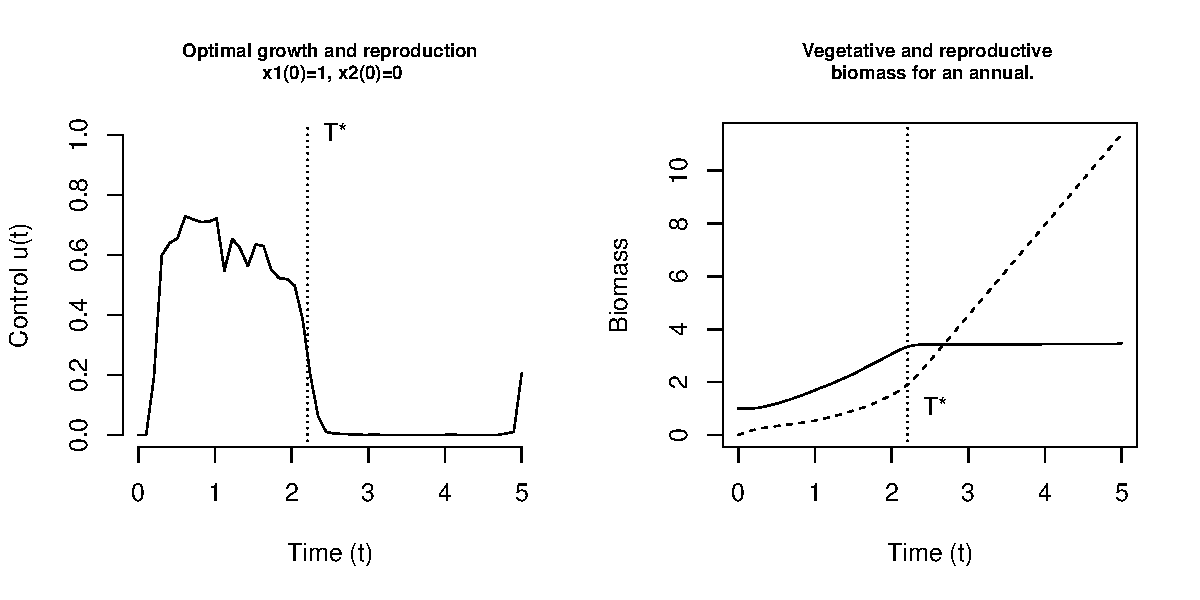
\includegraphics[page=1,width=.9\textwidth]{../../king-roughgarden/controlTrajectory-x1-1-x2-0}  
    \caption{ (A) The left panel shows the control $u(t)$ that maximizes $ \int_{0}^{T} log(x_2) dt. $ Here, $ T=5$ and $x_2(0)/x_1(0) = 0$. (B) The right panel shows the solution to the ODE for the control $u(t)$. [This figure corresponds to Figure 3 in King and Roughgarden (1982).] }
 \label{fig:kingRoughgardenFigure3}
\end{figure}

 \begin{figure}[h]
   \centering
       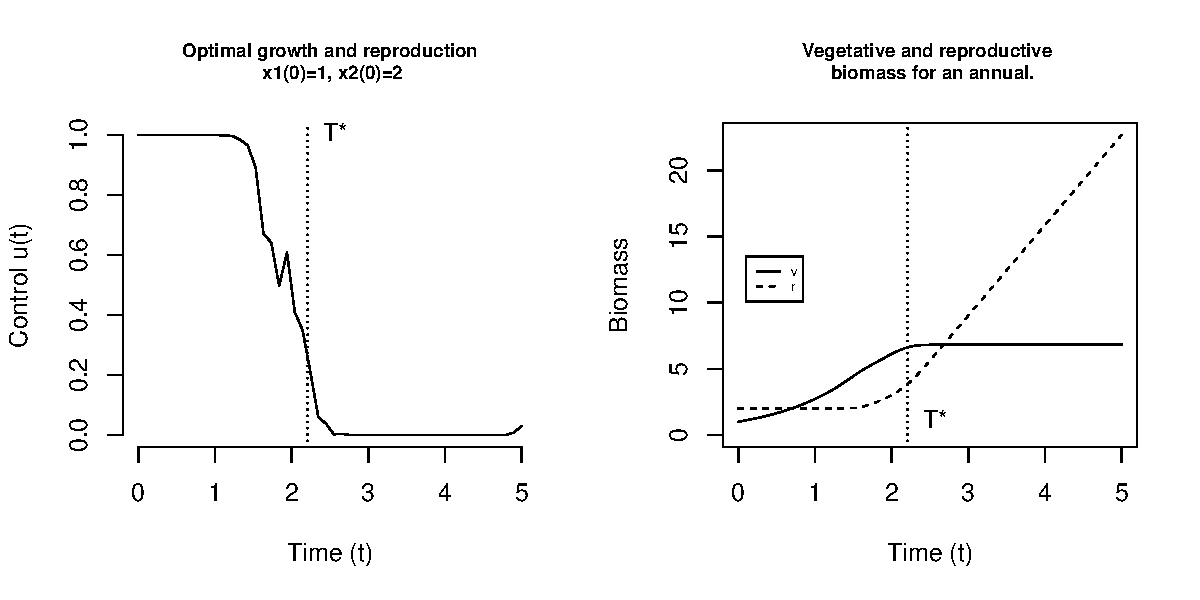
\includegraphics[page=1,width=.9\textwidth]{../../king-roughgarden/controlTrajectory-x1-1-x2-2}  
    \caption{ (A) The left panel shows the control $u(t)$ that maximizes $ \int_{0}^{T} log(x_2) dt. $ Here, $ T=5$ and $x_2(0)/x_1(0) = 2.0$. (B) The right panel shows the solution to the ODE for the control $u(t)$. [This figure corresponds to Figure 4 in King and Roughgarden (1982).] }
 \label{fig:kingRoughgardenFigure4}
\end{figure}

 \begin{figure}[h]
   \centering
       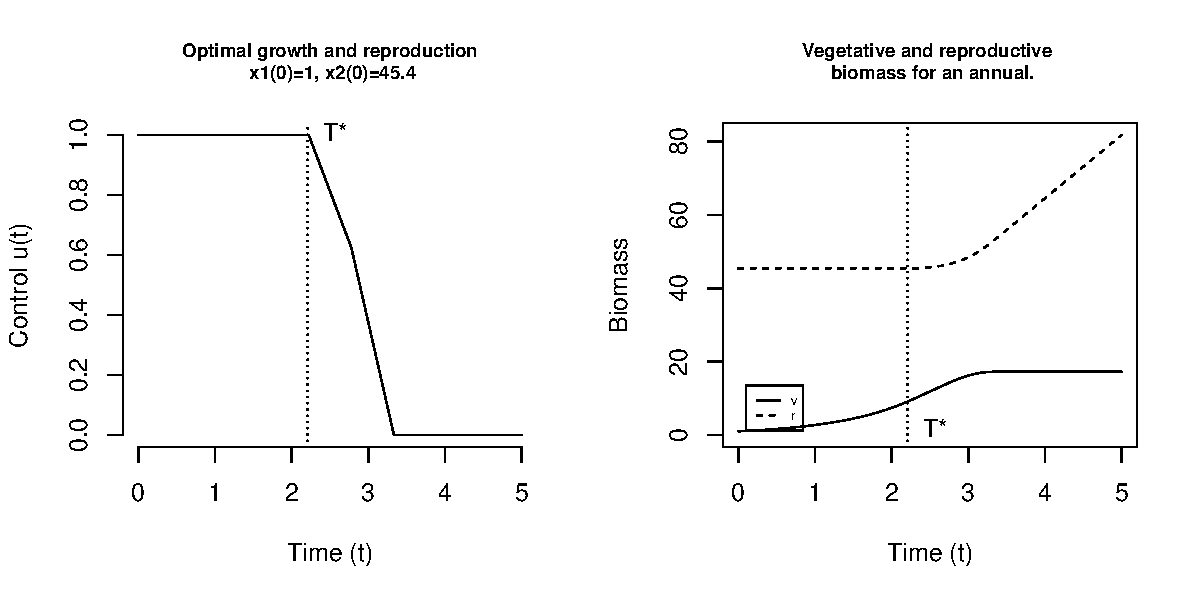
\includegraphics[page=1,width=.9\textwidth]{../../king-roughgarden/controlTrajectory-x1-1-x2-454}  
    \caption{ (A) The left panel shows the control $u(t)$ that maximizes $ \int_{0}^{T} log(x_2) dt. $ Here, $ T=5$ and $x_2(0)/x_1(0) = 2.0$. (B) The right panel shows the solution to the ODE for the control $u(t)$. [This figure corresponds to Figure 5 in King and Roughgarden (1982).] }
 \label{fig:kingRoughgardenFigure5}
\end{figure}

\end{document}